% !TEX encoding = UTF-8 Unicode
\documentclass[
11pt,
master, % тип документа
subf, % подключить и настроить пакет subfig для вложенной нумерации рисунков
href, % подключить и настроить пакет hyperref
colorlinks=true, % цветные гиперссылки
%fixint=false % отключить прямые знаки интегралов
]{disser}
\usepackage[left=25mm, top=20mm, right=10mm, bottom=20mm]{geometry}
\usepackage[T2A]{fontenc}
\usepackage[utf8]{inputenc}
\usepackage[english,russian]{babel}
\usepackage{amsmath,amssymb,cmap} % cmap для кодировки шрифтов в pdf
\usepackage{pdfpages} % вставляем pdf файлы
\usepackage{indentfirst} % отделять первую строку раздела абзацным отступом
\usepackage{titletoc} % убираем отступ перед "Оглавление"
\usepackage{graphicx}
\usepackage{setspace}
\usepackage{verbatim} % для оформления кода
\usepackage{pdfsync} % установка соответствия документ - код
\graphicspath{{./Img/}}

\setlength\parindent{5ex} % абзацный отступ равный пяти строчным буквам основного шрифта
\setcounter{tocdepth}{2} % включать подсекции в оглавление
\linespread{1.3} % полуторный интервал

\pagestyle{footcenter}
\chapterpagestyle{footcenter}

\begin{document}
\pagestyle{empty}
\begin{center}
	
	\noindent  Федеральное государственное бюджетное образовательное учреждение\\
	высшего профессионального образования\\
	
	Московский государственный технический университет им. Н.Э. Баумана \\
	Факультет <<Фундаментальные науки>>\bigskip\\
	
	\vfill
	
	Лабораторная работа №1\\
	по курсу «Вычислительная физика»\\
	
	
	\vfill
	\vfill
	\begin{flushright}
		\begin{tabular}{ll}
			Выполнил: & студент группы ФН4-82Б     \\
			& Хижик А.И. \\
			Проверил:  & доцент, к.физ.-мат.н.       \\
			& Хасаншин Р.Х.
		\end{tabular}
	\end{flushright}
	\vfill
	\begin{center}
		Москва, $2020$
	\end{center}
	
\end{center}
\pagebreak


\pagestyle{plain}
\tableofcontents

\section{Теоретическая часть}
\subsection{Моделирование траекторий нейтронов и фотонов}

Реализация метода Монте-Карло при решении задач переноса излучения сводится к процессу моделированию траекторий частиц в среде, который состоит из следующих основных этапов:

\begin{itemize}
\item Розыгрыша параметров источника;
\item Розыгрыша длины свободного пробега;
\item Розыгрыша типа взаимодействия;
\item Розыгрыша параметров частицы после взаимодействия.
\end{itemize}

Рассмотрим более подробно отдельные этапы моделирования распространения незаряженных частиц.

\subsubsection{Розыгрыш параметров источника}

Моделирование траектории начинается с определения координат рождения частицы $\vec{r}_{0} $, направления ее движения $\vec{\Omega }_{0} $ и энергии $E_{0} $. Для нормированной на единицу функции распределения источника
\[
\int d \vec{r}\int d \vec{\Omega }\int dE q\left(\vec{r},E,\vec{\Omega }\right)=1
\]
вероятность появления $\vec{r}_{0} $ в элементе объёма $d\vec{r}$:
\begin{equation} \label{GrindEQ__2_}
P\left(\vec{r}_{0} \in d\vec{r} \right)=d\vec{r}\iint q \left(\vec{r},E,\vec{\Omega } \right) dEd\vec{\Omega }=q \left(\vec{r} \right)d\bar{r},
\end{equation}
а так же условные вероятности попадания $\vec{\Omega }_{0} $ в $d\vec{\Omega }$
\begin{equation} \label{GrindEQ__3_}
P \left(\vec{\Omega }_{0} \in d\vec{\Omega }\left|\vec{r}_{0} \right. =\vec{r} \right)=\frac{\int dE q \left(\vec{r},E,\vec{\Omega } \right)}{\iint q \left(\vec{r},E,\vec{\Omega } \right) dEd\vec{\Omega }} d\vec{\Omega }=\frac{q \left(\vec{r},\vec{\Omega } \right)}{q \left(\vec{r} \right)} d\vec{\Omega }
\end{equation}
и энергии $E_{0} $ в $dE$
\begin{equation} \label{GrindEQ__4_}
P \left(E_{0} \in dE \mid \vec{r}_{0} =\vec{r},\vec{\Omega }_{0} =\vec{\Omega } \right) = \frac{q \left(\vec{r},E,\vec{\Omega } \right)}{\int dE q \left(\vec{r},E,\vec{\Omega } \right)} dE=\frac{q \left(\vec{r},\vec{\Omega },E \right)}{q \left(\vec{r},\vec{\Omega } \right)} dE.
\end{equation}
Перемножив \eqref{GrindEQ__2_}-\eqref{GrindEQ__4_}, получим
\begin{equation} \label{GrindEQ__5_}
P \left(\vec{r}_{0} \in d\vec{r} \right)P \left(\vec{\Omega }_{0} \in d\vec{\Omega } \mid \vec{r}_{0}  =\vec{r} \right)P \left(E_{0} \in dE \mid \vec{r}_{0} =\vec{r},\vec{\Omega }_{0} =\vec{\Omega } \right)=q \left(\vec{r},E,\vec{\Omega } \right)d\vec{r}dEd\vec{\Omega },
\end{equation}
т.е. выбрав последовательно $\vec{r}_{0},  E_{0}, \vec{\Omega }_{0} $ из распределений
\begin{equation} \label{GrindEQ__6_}
p_{\vec{r}_{0} } \left(\vec{r})=q(\vec{r} \right), ~~ p_{\vec{\Omega }_{0} } \left( \vec{\Omega } \mid \vec{r}_{0} \right) = \frac{q \left(\vec{r}_{0} ,\vec{\Omega } \right)}{q \left(\vec{r}_{0} \right)}, ~~ p_{E_{0} } \left(E \mid \vec{r}_{0} ,\vec{\Omega }_{0} \right)=\frac{q \left(\vec{r}_{0} ,\vec{\Omega }_{0} ,E \right)}{q \left(\vec{r}_{0} ,\vec{\Omega }_{0} \right)} ,
\end{equation}
найдем совокупность случайных величин $\left(\vec{r}_{0}, E_{0},  \vec{\Omega }_{0} \right)$ с распределением $q \left(\vec{r},\vec{\Omega },E \right)$. Если переменные в функции источника разделяются (независимые)
\[q \left(\vec{r},E,\vec{\Omega } \right)=q_{1} \left(\vec{r} \right)q_{2} (E)q_{3} \left(\vec{\Omega } \right),\]
 то соответствующие случайные величины моделируются независимо друг от друга.

Рассмотрим изотропный источник моноэнергетических частиц, равномерно распределенный по круговой подложке радиусом $R$, т.е. все переменные разделяются. В данном случае удобно воспользоваться полярной системой координат.

В силу симметрии, плотность вероятности вылета частиц из источника на расстоянии  $\rho $ от центра в интервале $d\rho $ будет пропорциональна площади кольца  $f(\rho )d\rho \approx 2\pi \rho d\rho $,
\[f(\rho )=\frac{2\pi \rho }{\int _{0}^{R}2\pi \rho d\rho  } =\frac{2\rho }{R^{2} } .\]
Следовательно, функция распределения
\[F(\rho )=\int _{0}^{\rho }f \left( \rho ' \right)d\rho '=\frac{\int _{0}^{\rho }2 \rho 'd\rho '}{R^{2} } =\frac{\rho ^{2} }{R^{2} } =\gamma .\]
Применяя метод обратных функций, получаем $F(\rho )=\gamma $ и $\rho =R\sqrt{\gamma } $. Точка вылета частицы для данного $\rho $ равновероятно распределена на промежутке $(0,2\pi )$ по азимутальному углу $\psi $, поэтому $f(\psi )=\frac{1}{2\pi } $ и $F(\psi )=\int _{0}^{\psi }f \left(\psi ' \right)d\psi '=\frac{\psi }{2\pi } =\gamma $ откуда получаем $\psi =2\pi \gamma $.

Разыграем направление вылета для  изотропного источника   $f \left(\vec{\Omega }_{0} \right)d\vec{\Omega }_{0} =\frac{d\vec{\Omega }_{0} }{4\pi } =\frac{d\cos \theta _{0} }{2} \frac{d\psi _{0} }{2\pi } $, т.е. величины $\cos \theta _{0} $ и $\psi _{0} $ распределены независимо и равномерно в интервалах $(-1,+1)$ и $(0,2\pi )$ соответственно. Применяя метод обратных функций, получаем
\[F(\cos \theta _{0} )=\int _{-1}^{\cos \theta _{0} }f(t)dt =\frac{1}{2} \int _{-1}^{\cos \theta _{0} }dt =\frac{\cos \theta _{0} +1}{2} =\gamma, \quad \cos \theta _{0} =2\gamma -1.\]
Вследствие азимутальной симметрии угол $\psi _{0} $ можно разыгрывать по формуле $\psi _{0} =2\pi \gamma $, но на практике экономичнее разыгрывать значения косинуса и синуса этого угла, потому что именно они используются для дальнейших расчётов. С помощью метода исключения косинусы и синусы моделируются как координаты единичного изотропного вектора на плоскости по схеме:
\begin{enumerate}
  \item $a=1-2\gamma _{1} ,\quad b=1-2\gamma _{2}$;
  \item $d=a^{2} +b^{2} $, если $d>1$, то возвращаемся к пункту 1, иначе -- на 3;
  \item $\cos \psi _{0} =\frac{a}{\sqrt{d} }, \quad \sin \psi _{0} =\frac{b}{\sqrt{d}}$.
\end{enumerate}

В рассмотренном примере все распределения имеют простой вид, что редко встречается на практике, поэтому выбор оптимальных алгоритмов обычно представляет собой не простою задачу.

\subsection{Розыгрыш длины свободного пробега}

Розыгрыш длины свободного пробега вдоль заданного направления $\vec{\Omega }$ является следующим шагом после выбора параметров источника. Для однородной изотропной среды розыгрыш производим методом обратной функции. Плотность распределения случайной величины $L$ определяется транспортным ядром интегрального уравнения переноса. Поэтому плотность и функцию распределения  длины свободного пробега в направлении $\vec{\Omega }$ можно записать в виде
\[f_{L} (t)=\Sigma [\vec{r}(t),E]\exp [-\tau (t,E)],\]
\[F_{L} (t)=1-\exp [-\tau (t,E)],\quad t>0,\]
где $\vec{r}(t)=\vec{r}'+t\, \vec{\Omega }$; $\tau (t,E)=\int _{\, 0}^{\, t}\Sigma \left[\vec{r}(t'),E \right] \, dt'$.

Получим случайную величину $L$ для незаряженной частицы в однородной бесконечной среде, плотность распределения которой равна
\[f_{L} (x)=\left\{\begin{array}{l} {\Sigma (E)\exp [-\Sigma (E)x],\quad x\ge 0,} \\ {0,\quad \quad \quad \quad \, \, \, x<0.} \end{array}\right.\]
Для этого решаем уравнение
\[\int _{0}^{L}f_{L}  (x)dx=1-\exp [-\Sigma (E)L]=\gamma ,\]
отсюда
$$L=-\frac{1}{\Sigma (E)} \ln (1-\gamma )\;\text{или}\;L=-\frac{1}{\Sigma (E)} \ln \gamma,$$
так как случайные величины $\gamma $ и $1-\gamma $ статистически эквивалентны, то получаем выражение для розыгрыша длины свободного пробега в однородной среде
\[L=-\ln \frac{\gamma}{\Sigma (E)}.\]


\subsection{Розыгрыш типа взаимодействия}

Следующий шаг заключается в розыгрыше типа взаимодействия. Пусть полное поперечное сечение для  $i$-го атома
\[\sigma _{i} =\sum _{\, k=1}^{\, m}\sigma _{ik}  ,\]
где $\sigma _{ik} $ -- парциальное сечение для $k$-го типа взаимодействия с $i$-атомом. Введя дискретную случайную величину $\eta $, принимающую значения от 1 до $m$ с вероятностью $p_{k} =\frac{\sigma _{ik} }{\sigma _{i} } $, т.е. имеющую распределение вида  $\eta =\left(\begin{array}{l} {1\, \quad \, 2\, \; \, \ldots \, \, \; m} \\ {p_{1} \, \, \, p_{2} \; \, \ldots \, \; p_{m} } \end{array}\right)$.  Разыгрываем значения $\eta $ и определяем тип  взаимодействия на $i$-м атоме, по следующей схеме:
\begin{enumerate}
\item  если  $\gamma \le \frac{\sigma _{i1} }{\sigma _{i} } $, то произошло взаимодействие 1-го типа с атомом \textit{k}-го типа;

\item  если  $\gamma >\frac{\sigma _{i1} }{\sigma _{i} } $, то проверяется выполнение следующего неравенства
$$
\frac{\sum _{\, k=1}^{\, l}\sigma _{ik}  }{\sigma _{i} } <\gamma \le \frac{\sum _{\, k=1}^{\, l+1}\sigma _{ik}  }{\sigma _{i} } , ~~ \eta =l+1.
$$
\end{enumerate}

Если последнее неравенство выполняется при некотором $l$, то полагают, что произошло взаимодействие ($l+1$)-го типа.

Далее мы будем рассматривать задачу переноса фотонов с учетом следующих типов взаимодействий: рассматривается комптоновское рассеяние, фотоэффект, образование электронно-позитронной пары, когерентное рассеяние и образование фотонейтронов. В таком случае полное сечение взаимодействия фотонов есть сумма сечений упомянутых выше процессов
$$
\Sigma =\sigma _{K} +\sigma _{\Phi} +\sigma _{n} +\sigma _{el} +\sigma _{\gamma ,n} ,
$$

Параметры после столкновения включают энергию и направление движения рассеянной первичной частицы, а также тип, число, энергию и направление движения любых вторичных частиц, родившихся при взаимодействии. Эти параметры определяются с помощью ядра столкновений и предполагают использование данных по дифференциальным поперечным сечениям, причём более подробных, чем при выборе типа взаимодействия.

Если произошёл фотоэффект, и нас не интересует история фотоэлектрона, то мы переходим к следующему фотону из заданной статистики. Если же произошло комптоновское рассеяние, то мы вынуждены рассматривать историю рассеянного фотона, предварительно определив энергию фотона и направление его движения. При комптоновском рассеянии, фотон с первоначальной энергией $E'$ в результате взаимодействия с электроном передаёт ему часть энергии и изменяет направление своего движения. Поскольку скорость атомных электронов очень мала по сравнению со скоростью света, то можно считать электрон свободным и покоящимся.


Энергия рассеянного фотона и угол рассеяния связаны формулой $E= \frac{E'}{1+E'(1-\cos \theta )/mc^{2}}$. Введя обозначения $\alpha =\frac{E}{m_{0} c^{2}} $ и $\alpha '=\frac{E'}{m_{0} c^{2} } $, получим выражение энергии рассеянного фотона в единицах энергии массы покоя электрона
$\alpha =\frac{\alpha '}{1+\alpha '(1-\cos \theta )}.$

Рассмотрим выбор энергии и направления движения фотона после комптоновского рассеяния. Из приведённого выше выражения следует, что потеря энергии и косинус угла рассеяния жёстко связаны между собой, достаточно разыграть одну из этих величин. Приведем один из возможных алгоритмов, основанный на методе исключения. Плотность распределения энергии после рассеяния $\alpha $ пропорциональна функции
\[
f(x,\alpha ')\sim p(x,\alpha ')=\frac{x}{\alpha '} +\frac{\alpha '}{x} + \left(\frac{1}{\alpha '} -\frac{1}{x} \right) \left(2+\frac{1}{\alpha '} -\frac{1}{x} \right),
\]
при $\frac{\alpha '}{1+2\alpha '} <x<\alpha '$.

Следовательно, справедливо соотношение
\[p(x,\alpha ')\le 1+2\alpha '+\frac{1}{1+2\alpha '} \]
Величину $\alpha $ определяем с помощью метода исключения:
\begin{description}
  \item[a.] выберем два значения $\gamma _{1} $, $\gamma _{2} $ случайной величины  $\gamma $ равномерно распределённой на интервале $(0,1)$;
  \item[b.] вычислим $x=\frac{\alpha ' \left(1+2\alpha '\gamma _{1} \right)}{1+2\alpha '} $, и отсюда находим $p \left(x,\alpha ' \right)$
  \item[c.] если при этом $\gamma _{2} \left(1+2\alpha '+\frac{1}{1+2\alpha '} \right)<p(x,\alpha ')$, то $\alpha =x$, иначе снова выполняется п. a) и т. д.
\end{description}

После определения энергии, определяют направление движения после взаимодействия. Азимутальный угол рассеяния выбирается из равномерного распределения по схеме приведённой выше, а косинус угла рассеяния рассчитывается по формуле  $\mu _{s} =\cos \theta _{s} =1-1/\alpha +1/\alpha '$.

В декартовой системе координат новое направление движения задаётся тремя направляющими косинусами
$$\vec{\Omega }=\vec{i}\cos x+\vec{j}\cos y+\vec{k}\cos z~\text{или}~\vec{\Omega }=\vec{i}\omega _{1} +\vec{j}\omega _{2} +\vec{k}\omega _{3}.$$
Формулы перехода от $\vec{\Omega }'$ к $\vec{\Omega }$ выглядят следующим образом:
$$
\omega _{3} =\omega '_{3} \mu _{s} +\sqrt{ \left(1-\mu _{s}^{2} \right) \left[1- \left(\omega '_{3} \right)^{2} \right]} \cos \psi _{s};
$$
$$
\omega _{2} =\frac{\omega '_{2} \left(\mu _{s} -\omega '_{3} \omega _{3} \right)+\omega '_{1} \sin \psi \sqrt{\left(1-\mu _{s}^{2} \right) \left[1-(\omega '_{3} )^{2} \right]} }{1-\left(\omega '_{3} \right)^{2} };
$$
$$
\omega _{1} = \frac{\omega '_{1} \left(\mu _{s} -\omega '_{3} \omega _{3} \right)-\omega '_{2} \sin \psi \sqrt{\left(1-\mu _{s}^{2} \right)[1-\left(\omega '_{3} \right)^{2} ]} }{1-\left(\omega '_{3} \right)^{2} }.
$$

Разыгрывая длину свободного пробега после первого столкновения
$$L_{2} =-\frac{\ln \xi }{\Sigma (E_{2} )} $$ 
находим точку $\vec{r}_{2} =\vec{r}_{1} +L_{2} \vec{\Omega }_{2} $

Координаты точки $(n+1)$-го взаимодействия находятся в декартовой системе координат по формулам:
$$x_{n+1} =x_{n} +L_{n+1} \omega _{1,n} ;$$
$$y_{n+1} =y_{n} +L_{n+1} \omega _{2,n} ;$$
$$z_{n+1} =z_{n} +L_{n+1} \omega _{3,n} .$$

Зная энергию рассеянного фотона можно вычислить сечение его последующего взаимодействия с веществом (полное или комптоновского взаимодействия).

В процессе комптоновского взаимодействия фотоны рассеиваются под всевозможными углами $(0 \le \theta_{s} \le \pi )$, и дифференциальное угловое сечение рассеяния (т.е. отнесённое к единице телесного угла) при этом, рассчитывается на основании квантовой электродинамики и выражается формулой Клейна-Нишины-Тамма:
\begin{equation} \label{GrindEQ__16_}
\sigma _{C} \left(\alpha ',\theta _{s} \right)=\frac{Zr_{e} ^{2} }{2} \left[1+\alpha '(1-\mu _{s} )\right]^{-2} \left[1+\mu _{s} ^{2} +\frac{\left(\alpha ' \right)^{2} (1-\mu _{s} )^{2} }{1+\alpha '(1-\mu _{s} )} \right],
\end{equation}
где $Z$ -- атомный номер материала среды; $r_{e}$ -- классический радиус электрона.

Для фотонов высоких энергий наблюдается преимущественное рассеяние вперед, а с уменьшением энергии дифференциальное сечение имеет все более плавную угловую зависимость, и в пределе при $\alpha '\to 0$ из выражения \eqref{GrindEQ__16_} получаем классическую формулу Томсона (см${}^{2}$/ср):
\[
\sigma _{s} \left(\theta _{s} \right) = Zr_{e} ^{2} \left(1+\cos ^{2} \theta _{s} \right)/2.
\]

Интегрирование формулу \eqref{GrindEQ__16_} по телесному углу даёт выражение (согласно теории Клейна-Нишины-Тамма) для полного сечение комптоновского взаимодействия фотонов со свободными электронами имеет вид
\begin{equation} \label{GrindEQ__17_}
\sigma _{C} (\alpha ')=2\pi Zr_{e}^{2} \left\{\frac{1+\alpha '}{\alpha '^{2} } \left[\frac{2(1+\alpha ')}{1+2\alpha '} -\frac{\ln (1+2\alpha ')}{\alpha '} \right]+\frac{\ln (1+2\alpha ')}{2\alpha '} -\frac{1+3\alpha '}{(1+2\alpha ')^{2} } \right\}.
\end{equation}


\subsection{Локальная оценка потока}
\subsubsection{Оценки функционалов в методе Монте-Карло }
Рассмотрим, какие случайные величины (оценки) следует ввести в шестимерном фазовом пространстве траекторий $\Gamma $, чтобы их математические ожидания равнялись конкретному функционалу.

Пусть необходимо рассчитать линейный функционал
\begin{equation} \label{GrindEQ__18_}
I_{g} = \left(\psi, g \right) = \iint \limits _{\Gamma }\psi \left(\vec{r},\vec{E} \right) g \left(\vec{r},\vec{E} \right)d\vec{r}d\vec{E},
\end{equation}
где $g \left(\vec{r}, \vec{E} \right)$ -- функция отклика детектора, $\psi \left(\vec{r},\vec{E} \right)$ -- плотность столкновений, удовлетворяющая интегральному уравнению
\[
\psi \left(\vec{r},\vec{E} \right)=q_{1} \left(\vec{r},\vec{E} \right)+\iint K\left(\vec{r}',\vec{E}';\vec{r},\vec{E}\right)\psi \left(\vec{r}',\vec{E}' \right) d\vec{r}'d\vec{E}'.
\]

Далее предполагается, что любая траектория в рассматриваемых процессах случайного блуждания с вероятностью единица заканчивается после конечного числа соударений.

Построим процесс случайных блужданий (цепь Маркова) с параметрами $p_{1} (x)$, $p\left(x',x \right)$, $p(x)$, удовлетворяющий следующим условиям
\[\left. \begin{array}{l} {p_{1} (x)\ne 0,\;\, \text{при} \; \, q_{1} (x)\ne 0;} \\ {p(x',x)\ne 0,\;\, \text{при} \; \,  K(x',x)\ne 0;\quad } \\ {p(x)\ne 0,\;\, \text{при} \; \,  g(x)\ne 0.} \end{array}\right\}\]

Таким образом, траектории должны начинаться в тех точках, где $q_{1} (x)\ne 0$, а при переходе $x'\to x$ попадать в те точки где $K\left(x',x\right)\ne 0$.

\textbf{\textit{Определение.}} \textbf{\textit{Марковский процесс}}, процесс без последствий, -- случайный процесс, эволюция которого после любого заданного момента времени $t$ не зависит от эволюции предшествующей $t$, при условии, что значение процесса в этот момент фиксировано (короче: «будущее» и «прошлое»  процесса не зависят друг от друга при известном «настоящем»)

\textbf{\textit{Определение.}} \textbf{\textit{Марковская цепь}} - марковский процесс, с конечным или счётным множеством состояний.

\subsubsection{Оценка по столкновениям}
 Такая оценка рассчитывается во всех точках траектории $\alpha =(x_{1} ,\ldots ,x_{k} )$ и имеет вид
\begin{equation} \label{GrindEQ__19_}
\eta (\alpha )=\sum\limits_{m=1}^{k}W_{m}  (\alpha )g(x_{m} ),
\end{equation}
где $W_{m} $ -- вес частицы при \textit{m}-м столкновении, определяется из выражения
\begin{equation} \label{GrindEQ__20_}
W_{m} (\alpha )=\frac{q_{1} (x_{1} )}{p_{1} (x_{1} )} W(x_{1} ,x_{2} )\ldots W(x_{m-1} ,x_{m} ),
\end{equation}
где  $W(x',x)=\left\{\begin{array}{l} {K(x',x)/p(x',x),\quad p(x',x)\ne 0\, ;} \\ {0,\quad \quad \quad \quad \quad \quad \quad ~~ p(x',x)=0\, .} \end{array}\right. $

В теории метода Монте-Карло доказано, что $M\eta (\alpha )$ -- математическое ожидание случайной величины $\eta (\alpha )$ является несмещённой оценкой функционала $I_{g} =(\psi ,g)$.

\textbf{\textit{Определение}}. \textbf{\textit{Несмещённая оценка}} -- статистическая оценка, математическое ожидание которой совпадает с оцениваемой величиной.

\textbf{\textit{Определение}}. Если при расчёте по методу Монте-Карло точно моделируются реальные вероятностные законы, то такой способ расчёта называется аналоговым.

При аналоговом моделировании траектории частиц и при отсутствии деления в реакциях взаимодействия, учитывая, что $p_{1} (x)=q_{1} (x)$; $p(x',x)=K(x',x)$; $p(x)=\Sigma _{a} (x)/\Sigma (x)$, выражение для случайной величины $\eta (\alpha )$ принимает следующий вид\textbf{\textit{}}
\begin{equation} \label{GrindEQ__21_}
\eta (\alpha )=\sum _{\, m=1}^{\, k}g(x_{m} ) .
\end{equation}

Если, например, необходимо определить число реакций с сечением $\Sigma _{i} (x)$ в некотором объёме $V$, тогда функция отклика детектора
\[g(x)=\upsilon _{V} (x) \frac{\Sigma _{i} (x)}{\Sigma (x)} ,\]
где $\upsilon _{V} (x)$-- индикаторная функция объёма $V$, которая имеет вид
\[\upsilon _{V} (x)=\left\{\begin{array}{l} {1,\quad x\in V;} \\ {0,\quad x\notin V.} \end{array}\right. \]

Следовательно, выражение для оценки $\eta (\alpha )$ принимает вид
\begin{equation} \label{GrindEQ__22_}
\eta (\alpha )=\sum _{m=1}^{k}\frac{\Sigma _{i} (x_{m} )}{\Sigma (x_{m} )} \upsilon _{V} (x_{m} ) .
\end{equation}

\subsubsection{Локальная оценка потока}

Рассмотренная выше оценка $\eta (\alpha )$ даёт средние значения для функций $\psi \left(\vec{r},E\right)$, $\varphi \left(\vec{r},E\right)$ и функционалов от них по всей области регистрации частиц. Если градиент поля излучения достаточно велик, то чтобы уменьшить погрешность, связанную с усреднением, размеры области приходится уменьшать. Действительно детектор малых размеров практически не возмущает поле излучения, но обладает малой эффективностью, поэтому уменьшается вероятность попадания частицы в данную область, следовательно, увеличивается статистическая погрешность оценки. В таких случаях часто прибегают к локальным оценкам, позволяющим стягивать область детектирования в точку.

Рассмотрим, для простоты, распространение частиц в среде без размножения и поглощения, так как эти реакции учитываются с помощью весовых множителей. Пусть требуется оценить плотность потока частиц в точке фазового пространства $x^{*} =\{ \vec{r}^{*} ,E^{*} ,\vec{\Omega }^{*} \} $. Подставим эту точку в уравнение для плотности столкновений, приравняв для упрощения выражения $q_{1} (x^{*} )=0$:
\begin{equation} \label{GrindEQ__23_}
\psi (x^{*} )=\int K \left(x',x^{*} \right)\,  \psi \left(x' \right)dx'.
\end{equation}
Поделив обе части выражения \eqref{GrindEQ__23_} на $\Sigma _{s} (x^{*} )$, получим
\begin{equation} \label{GrindEQ__24_}
\varphi (x^{*} )=\int \frac{K\left(x',x^{*} \right)}{\sum _{s} (x^{*} )} \,  \psi (x')dx'.
\end{equation}
Формально функция $\varphi (x^{*} )$ представлена в виде функционала от плотности столкновений $\psi (x')$ с функцией отклика детектора, равной
$g \left(x',x^{*} \right)=\dfrac{K \left(x',x^{*} \right)}{\sum _{s} (x^{*} )}$
Для расчёта $\varphi (x^{*} )$ выберем оценку по столкновениям \eqref{GrindEQ__19_} и получим что математическое ожидание случайной величины
\begin{equation} \label{GrindEQ__25_}
\eta _{1} (\alpha )=\sum _{m=1}^{k}\frac{W_{m} (\alpha )}{\sum _{s} (x^{*} )} K(x_{m} ,x^{*} )
\end{equation}
равно плотности потока рассеянного излучения в точке $x^{*} $. Величину $W_{m} $-часто называют весом \textit{m-}го рассеяния. Она представляет собой условную вероятность «выживания» частицы испытавшей рассеяния в точках $(x_{1} ,\ldots ,x_{m} )$.  Определение плотности потока нерассеянного излучения в точке $x^{*} $, т.е. величины  $q_{1} (x^{*} )/\sum_{s} (x^{*} )$, как правило, не представляет особого труда и вычисляется аналитически с использованием выражения для источника первых столкновений
$q_{1} \left(\vec{r}^{*} ,\vec{E} \right)=\int d\vec{r} 'q \left(\vec{r}',\vec{E} \right)\cdot T\left(\vec{r}',\vec{r}^{*} \mid \vec{E} \right).$

Ядро $K \left(x_{m} ,x^{*} \right)$ содержит $\delta $-функцию, для устранения которой достаточно проинтегрировать \eqref{GrindEQ__24_} по некоторой области направлений $\Delta \vec{\Omega }_{i}^{*} $. Для локальной оценки плотности потока рассеянных фотонов (без учета когерентного рассеяния), движущихся в интервале $\Delta \vec{\Omega }_{i}^{*} $ с энергией в интервале $\Delta E_{i}^{*} $, в точке $\vec{r}^{*} $ окончательное выражение имеет вид
\begin{equation} \label{GrindEQ__26_}
\eta _{1} (\alpha )=\sum _{m=1}^{k}W_{m}  (\alpha )\frac{\exp \left[-\tau \left(\vec{r}_{m} ,\vec{r}^{*} ,E_{m}^{*} \right)\right]}{\left(\vec{r}_{m} -\vec{r}^{*} \right)^{2} } \frac{\sigma _{C} \left(\vec{r}_{m} ,E_{m} \to E_{m}^{*} ,\left(\vec{\Omega }_{m} \cdot \vec{\Omega }_{m}^{*} \right)\right)}{\sigma _{C} \left(\vec{r}_{m} ,E_{m} \right)} \Delta \left(E_{m}^{*} ,\Delta E_{i}^{*} \right)\Delta \left(\vec{\Omega }_{m}^{*} ,\Delta \vec{\Omega }_{i}^{*} \right),
\end{equation}
где $\tau \left(\vec{r}_{m} ,\vec{r}^{*} ,E_{m}^{*} \right)=\int _{\, }^{\vec{r}_{m} \to \vec{r}^{*} \, }\Sigma \left(\vec{r}''\left(t ,E_{m}^{*} \right) \right)dt$ -- оптическое расстояние между точками $\vec{r}_{m} $ и $\vec{r}^{*} $ для частицы с энергией $E_{m}^{*} $;
\[\Delta (x,\Delta x)=\left\{\begin{array}{l} {1,\quad x\in \Delta x\, ;} \\ {0,\quad x\notin \Delta x\, ;} \end{array}\right. \]
$\sigma _{C} \left(\vec{r}_{m} ,E_{m} \to E_{m}^{*} , \left(\vec{\Omega }_{m} \cdot \vec{\Omega }_{m}^{*} \right) \right)$, $\sigma _{C} \left(\vec{r}_{m} ,E_{m} \right)$ -- дифференциальное угловое сечение рассеяния и интегральное (полное) сечения комптоновского рассеяния.

Выражение \eqref{GrindEQ__26_} представляет собой локальную оценку плотности потока частиц. Если точка $\vec{r}^{*} $ не принадлежит области переноса излучения, то такая оценка имеет конечную дисперсию. В общем случае ее дисперсия расходится из-за множителя $1/\left(\vec{r}_{m} -\vec{r}^{*} \right)^{2} $. Это не является препятствием для ее использования в методе Монте-Карло, поскольку существования математического ожидания обеспечивает действие закона больших чисел. Сходимость среднего арифметического $\bar{\eta }_{N} $ (\textit{N} -- число историй) имеет порядок $N^{-1/3} $, а не $N^{-1/2} $, как это имеет место при конечной дисперсии. Иногда возможно появление выбросов в результатах расчётов, связанных с близостью некоторых точек столкновения к точке детектирования $\vec{r}^{*} $.

Математическое ожидание случайной величины $\eta _{1} (\alpha )$ равно плотности потока рассеянного излучения в точке $x^{*} $
\begin{equation} \label{GrindEQ__27_}
M\eta _{1} (\alpha )=\frac{1}{N} \sum _{l=1}^{N}\eta _{l}  (\alpha _{l} )=\varphi (x^{*} ),
\end{equation}
где \textit{N }-- статистика (число усредняемых траекторий).

Локальная оценка не позволяет рассчитывать угловую плотность потока в точке $\vec{r}^{*} $ непосредственно в заданном направлении $\vec{\Omega }^{*} $. Этого недостатка лишена двойная локальная оценка, функцию отклика детектора для которой берут в виде
\begin{equation} \label{GrindEQ__28_}
g_{1} \left(x',x^{*} \right)= \left(\int K \left(x',x'' \right)K \left(x'',x^{*} \right) \, dx''\right)/\sum _{s} x^{*}.
\end{equation}

Поясним смысл этой оценки. Если при локальной оценке производится, по существу, суммирование в точке детектирования виртуальных вкладов нерассеяного излучения непосредственно от точек столкновения, то при двойной локальной оценке суммируются виртуальные вклады в точке детектирования через промежуточную точку рассеяния.

Интеграл в выражении \eqref{GrindEQ__28_} берется по лучу $\vec{r}\; ''(t)=\vec{r}^{*} -\vec{\Omega }^{*} t,\quad t>0.$ Его можно оценить по одному случайному узлу $\vec{\rho }''$, который можно положить равным $\vec{\rho }''=\vec{r}^{*} -\vec{\Omega }^{*} L^{*} $, где $L^{*} $-- случайная длина свободного пробега из $\vec{r}^{*} $ в направлении обратном $\vec{\Omega }^{*} $. Математическое ожидание случайной величины
\begin{equation} \label{GrindEQ__30_}
\eta _{2} (\alpha )=\sum _{m=1}^{k}W_{m} \left(\alpha )g_{1} (x_{m} ,x^{*} \right)
\end{equation}
равно $M[\eta _{2} (\alpha )]=\varphi (x^{*} )-\varphi _{1} (x^{*} )-\varphi _{0} (x^{*} )$,
где $\varphi _{0} (x^{*} )$, $\varphi _{1} (x^{*} )$ -- плотность потока нерассеянного и однократно рассеянного излучения соответственно.

\textbf{Методы получения случайных чисел с заданным распределением}

Получения случайных чисел с заданным распределением называют \textit{розыгрышем} значений случайной величины.

Пусть случайная величина $\xi $, определена в интервале $(a,\, b)$ и имеет плотность распределения $f(x)$. \textit{Выборкой} из плотности $f(x)$ называется такая последовательность чисел $\{t_i\}$,  $(-\infty <t_{i} <+\infty )$, что:
\begin{enumerate}
  \item $p(a<t_{i} \le b)=\int _{\, a}^{\, b}f(x) dx,  (-\infty \le a<b\le +\infty );$
  \item $p \left(a<t_{i_{1} } ,\ldots ,t_{i_{n} } \le b \right)=\left[\int _{\, a}^{\, b}f(x) dx\right]^{n} $,  при условии, что все $i_{1} ,\ldots ,i_{n} $ различны.
\end{enumerate}

Наиболее распространённый способ получения таких последовательностей является использование последовательности чисел $\{\gamma_i\}$ представляющих собой выборочные значения случайной величины $\gamma $ равномерно распределённой на отрезке $[0,1]$. Такие числа представляют собой выборку из плотности распределения
$f(x)=\left\{\begin{array}{l} {1,\quad x\in [0,1];} \\ {0,\quad x\notin [0,1].} \end{array}\right. $

\subsubsection{Метод обратных функций}

Пусть случайная величина $\xi $, определена в интервале $(a,\, b)$ и имеет плотность распределения $f(x)>0$, $F(x)$ -- функция распределения.

Докажем, что выборочное значение $t$ случайной величины $\xi $, можно найти из уравнения
\begin{equation}\label{GrindEQ__0_}
  F(t)=\int _{\, a}^{\, t}f(x)\,  dx=\gamma\; \text{или}\;t=F^{-1} (\gamma ),
\end{equation}
где $F^{-1} $ -- обратная  функция.

Функция $F(x)$ строго возрастает в интервале $(a,\, b)$ от $F(a)=0$ до $F(b)=1$, поэтому уравнение \eqref{GrindEQ__0_} имеет единственный корень при каждом $\gamma $. При этом справедливо равенство вероятностей
\[P\{ x<t<x+dx\} =P\{ F(x)<\gamma <F(x+dx)\} ,\]
так как случайная величина $\gamma $ равномерно распределена в интервале $(0,1)$, то вероятность того, что ее значение окажется внутри интервала  $(F(x),F(x+dx))$, равна длине этого интервала
\[P\{ x<t<x+dx\} =F(x+dx)-F(x)=f(x)dx.\]
Следовательно, выборочное значение $t$ случайной величины $\xi $, имеет плотность распределения $f(x)$. Что и требовалось доказать.

Если $\{\gamma_i \}$ последовательность независимых чисел равномерно распределённых на промежутке $(0,1)$, то числа $t_{i} =F^{-1} (\gamma _{i} ), ~ i \in \mathbb{N}$ представляют собой выборку  из плотности распределения $f(x)$ для  $\xi =F^{-1} (\gamma )$.


В более общем случае, когда плотность распределения удовлетворяет условию $f(x)\ge 0$ в интервале $(a,\, b)$, то решением уравнения \eqref{GrindEQ__0_} является $t=\sup x$, при $F(x)<\gamma $.

\textit{Замечание.} Разыгрывание значений непрерывных случайных величин методом обратных функций требует существования аналитического решения уравнения \eqref{GrindEQ__0_} относительно $t$.

Рассмотрим дискретную случайную величину $\xi $, принимающую значения $x_{i} $ с вероятностями $p_{i}$. Выбор значения величины $\xi $ определим как и ранее  $t=\sup x_{i} $, при $F(x_{i} )<\gamma $.

Значению $\gamma $, удовлетворяющему неравенству
$\sum\limits_{i=0}^{j}p_{i}  <\gamma \le \sum\limits_{i=1}^{j+1}p_{i}  ,\; p_{0} =0,$
соответствует значение $\xi =x_{j+1} ,\; j \in \mathbb{N}$

Действительно, если обозначить интервал между $F(x_{j} )$ и $F(x_{j+1} )$ через $\Delta _{j+1} $, тогда $p\, (\xi =x_{j+1} )=p\, (\gamma \in \Delta _{j+1} )$.

\subsubsection{Метод равновероятных интервалов (табличный метод)}

Табличный метод основан на замене моделируемой случайной величины $\xi $ дискретной случайной величиной $\xi _{1} $, принимающей с равной вероятностью значения $x_{i}, \;i = \overline{1,n}$. До начала основного расчёта составляется таблица из $N$ равновероятных значений $x_{i} $ случайной величины $\xi _{1} $, функция распределения которой аппроксимирует функцию распределения случайной величины $\xi $. Для этого решается уравнение
 $$
 F(x_{i} )=\int _{\, -\infty }^{\, x_{i} }f(x)\, dx= \frac{2i-1}{2N} ,\quad i=\overline{1,n},
 $$ и строится таблица значений $i$ и соответствующих значений $x_{i} $. После этого для определения выборочного значения случайной величины $\xi _{1} $ достаточно получить случайное число $i$ принимающее с равной вероятностью значения от 1 до $N$, и выбрать из таблицы $x_{i} $.

\subsubsection{Метод исключения}

Метод исключения, так же как и метод равновероятных интервалов, свободен от недостатков метода обратных функций, связанных с необходимостью получения аналитического решения. Метод исключения, так же как и метод равновероятных интервалов, свободен от недостатков метода обратных функций, связанных с необходимостью получения аналитического решения. Кроме того, он не требует и предварительного расчёта таблиц.


Рассмотрим ограниченную на отрезке $[a,b]$ плотность распределения $f(x)$. Пусть $M=\sup f(x)$ и $f_{1} (x)=f(x)/M$, так что $0\le f_{1} (x)\le 1$. Используя пару равномерно распределённых на отрезке $[0,1]$  независимых случайных чисел $(\gamma _{1} ,\, \gamma _{2} )$, найдем координаты случайной точки $Q=\{ a+\gamma _{1} (b-a),\, \gamma _{2} \} $, лежащей в прямоугольнике с основанием $(b-a)$ и высотой 1. Если эта точка окажется под кривой $f_{1} (x)$, т. е. если $\gamma _{2} <f_{1} [a+(b-a)\, \gamma _{1} ]$, то $t=a+(b-a)\, \gamma _{1} $, принимается в качестве значения случайной величины  с плотностью распределения $f(x)$. В противном случае пара $(\gamma _{1} ,\, \gamma _{2} )$ отбрасывается, выбирается следующая пара $(\gamma _{3} ,\, \gamma _{4} )$ и все повторяется. Вычисленные по такому алгоритму значения $t$ распределены с условной плотностью вероятности
$f(t \mid \gamma _{2} <f_{1} (t))=\int _{\, 0}^{\, f_{1} (t)}g(t \mid \gamma _{2})d\gamma _{2}  \cdot \left[\int _{\, a}^{\, b}\left(\int _{\, 0}^{\, f_{1} (t)}g(t \mid \gamma _{2})d\gamma _{2}  \right) dt\right]^{-1}.$  Учитывая, что совместная плотность распределения  $g(t,\gamma _{2} )$ имеет вид
$$g(t,\gamma _{2} )=\left\{\begin{array}{l} {1/(b-a),\quad t\in [a,b],\quad \gamma _{2} \in [0,1]} \\ {0,\quad \quad \quad \quad~ t\notin [a,b],\quad \, \gamma _{2} \notin [0,1]} \end{array}\right.$$

Условная плотность распределения $g(t \mid \gamma _{2})$ совпадает с выражением для $g(t,\gamma _{2} )$, поэтому окончательно получаем
$$f(t\left|\gamma _{2} \right. <f_{1} (t))=\frac{1}{b-a}\int _{\, 0}^{\, f_{1} (t)}d\gamma _{2}  \cdot \left[\frac{1}{b-a}\int _{\, a}^{\, b}dt\left(\int _{\, 0}^{\, f_{1} (t)}d\gamma _{2}  \right) \right]^{-1} =f_{1} (t)\left[\int _{\, a}^{\, b}f_{1} (t) dt\right]^{-1} =f(t)$$
что и требовалось доказать.

\newpage
\section{Постановка задачи}
Плоский изотропный источник $\gamma$-квантов с энергиями $E_0 = 2.5$ МэВ в виде прямоугольника накрыт алюминиевым цилиндром. Геометрические центры основания цилиндра и прямоугольника совпадают. Радиус цилиндра $R_{\text{цил}} = 30$ см, высота цилиндра $H_{\text{цил}} = 20$ см. Стороны прямоугольника  равны соответственно $a = 40$ см, $b = 15$ см.
\begin{itemize}
\item Построить точки рождения частиц и нарисовать «ёжика» каждая игла, которого представляет собой отрезок соединяющий точку рождения $\gamma$-кванта с точкой его первого взаимодействия.
\item Методом локальной оценки потока вычислить распределения плотности потока рассеянных квантов вдоль оси симметрии задачи, образующей цилиндра и вдоль диаметров верхнего основания параллельных сторонам  прямоугольника $a$ и $b$.
\end{itemize}

\begin{figure}[htbp]
  \centering
  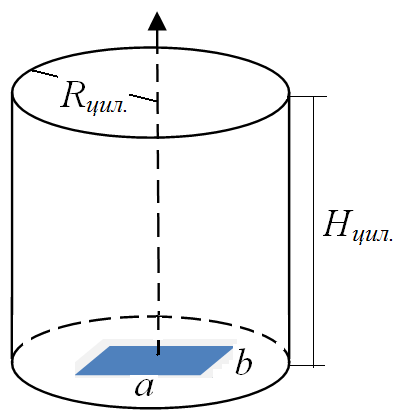
\includegraphics[width=0.5\linewidth]{pic1}
  \caption{}\label{}
\end{figure}

\newpage
\section{Результаты вычислений}
\begin{figure}[htbp]
\begin{minipage}[h]{0.3\linewidth}
\center{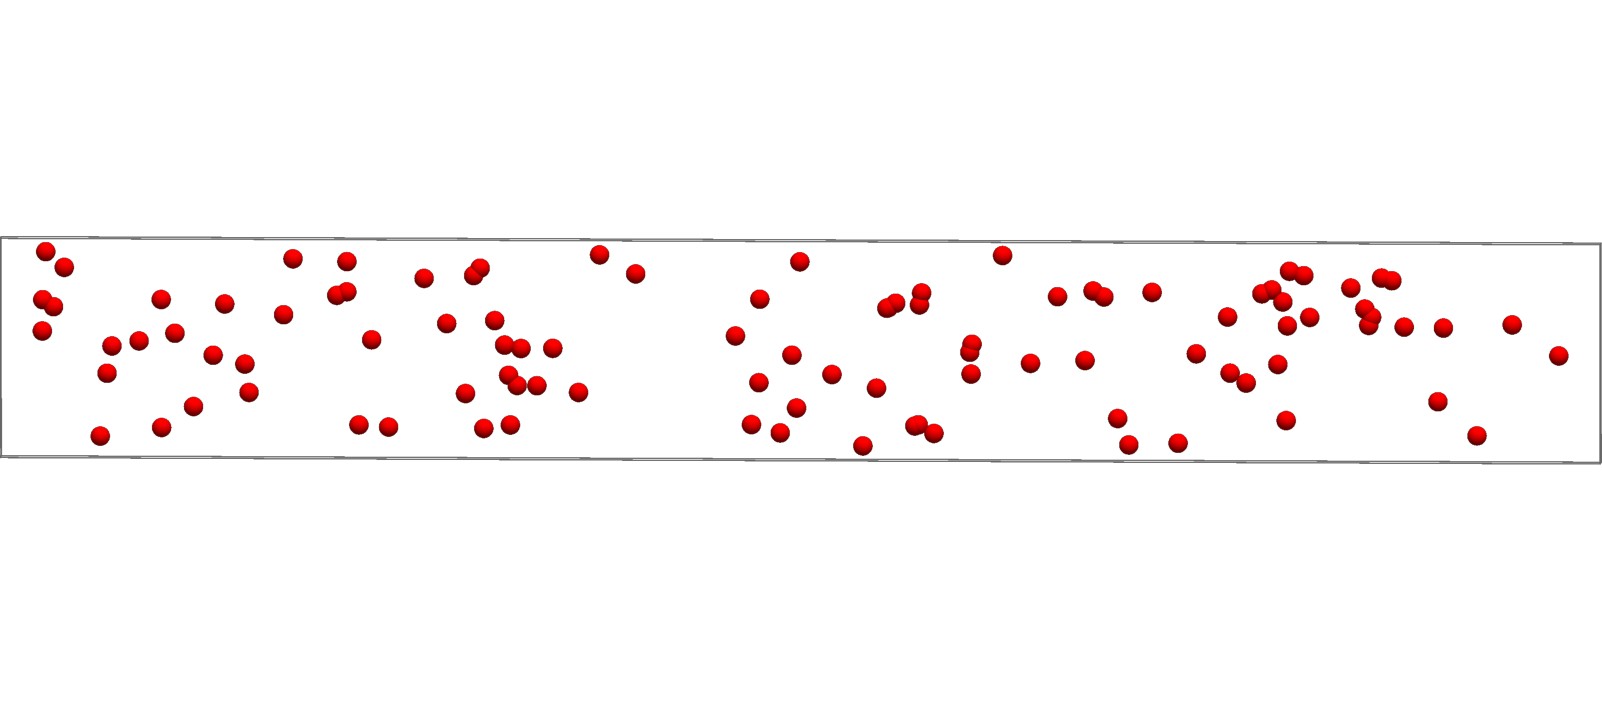
\includegraphics[width=1.3\linewidth]{Vis_200} \\ a)}
\end{minipage}
\hfill
\begin{minipage}[h]{0.68\linewidth}
\center{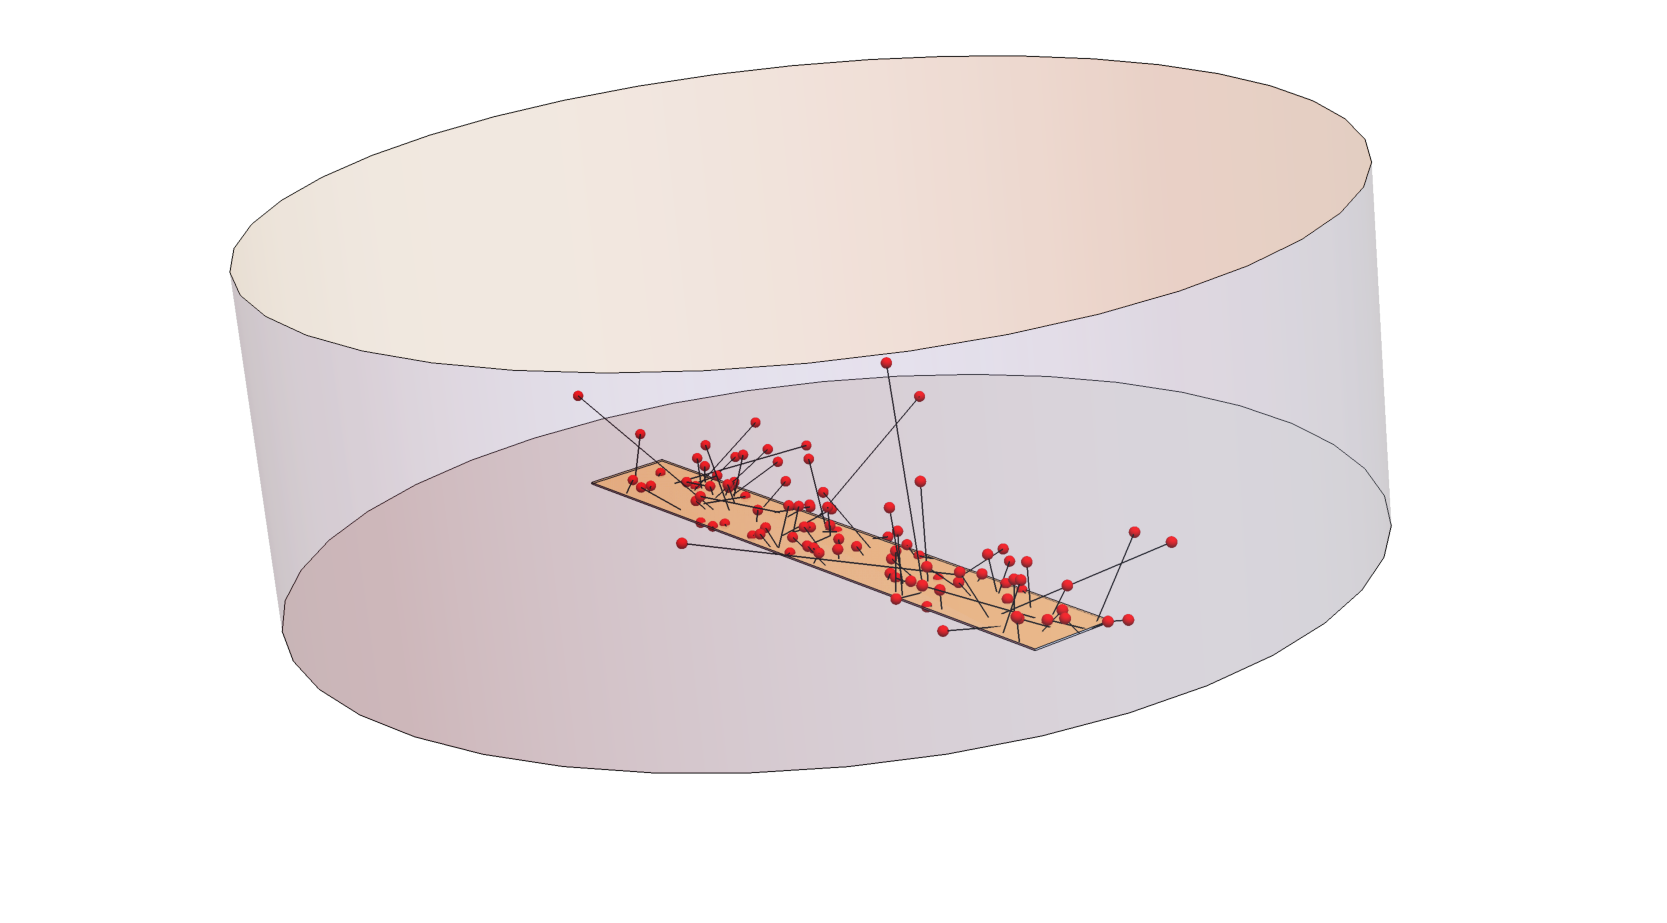
\includegraphics[width=1\linewidth]{Vis_200_1} \\ b)}
\end{minipage}
\caption{a) Точки рождения $\gamma$-квантов, b) <<Ёжик>>, $N = 200$}
\label{}
\end{figure}

\begin{figure}[htbp]
\begin{minipage}[h]{0.3\linewidth}
\center{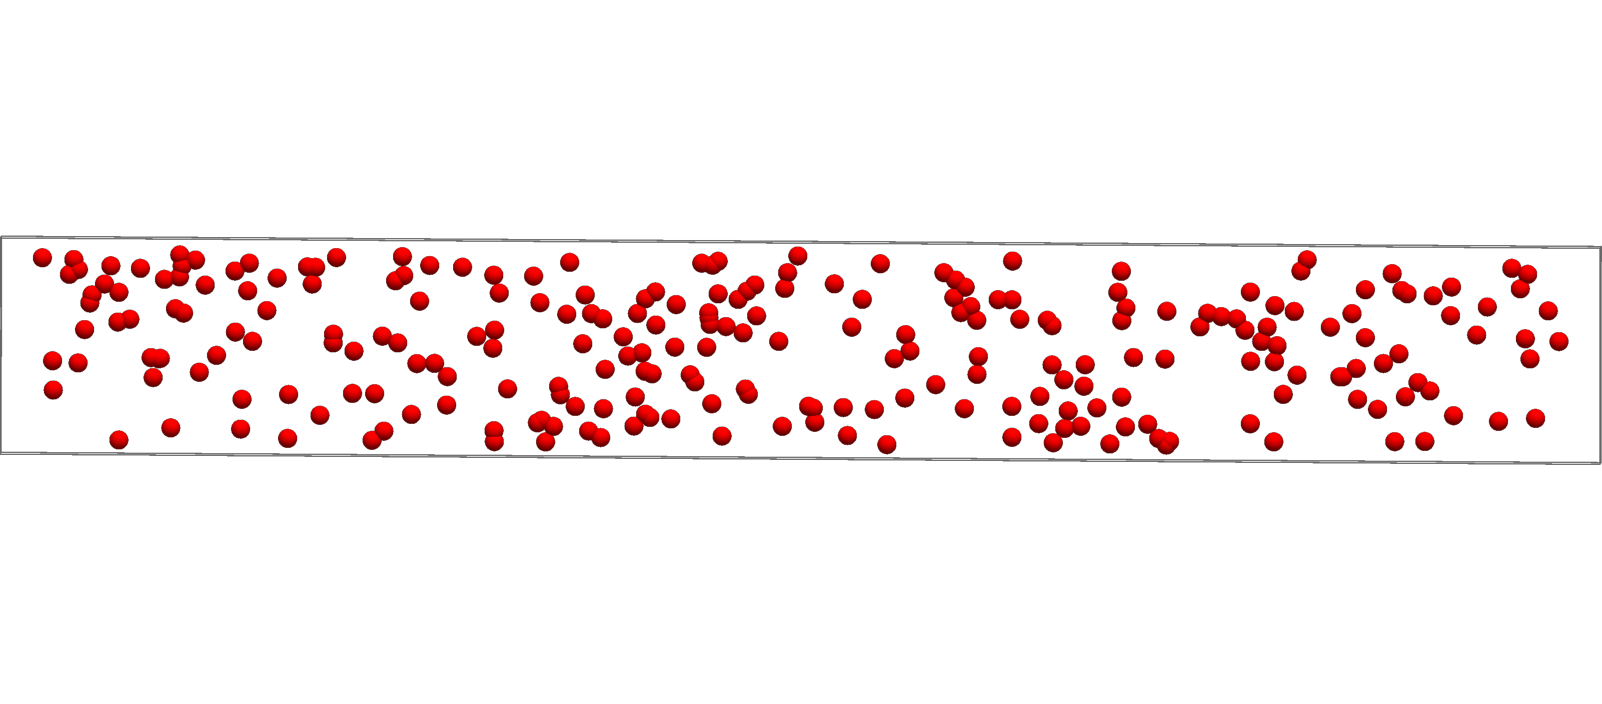
\includegraphics[width=1.3\linewidth]{Vis_500} \\ a)}
\end{minipage}
\hfill
\begin{minipage}[h]{0.68\linewidth}
\center{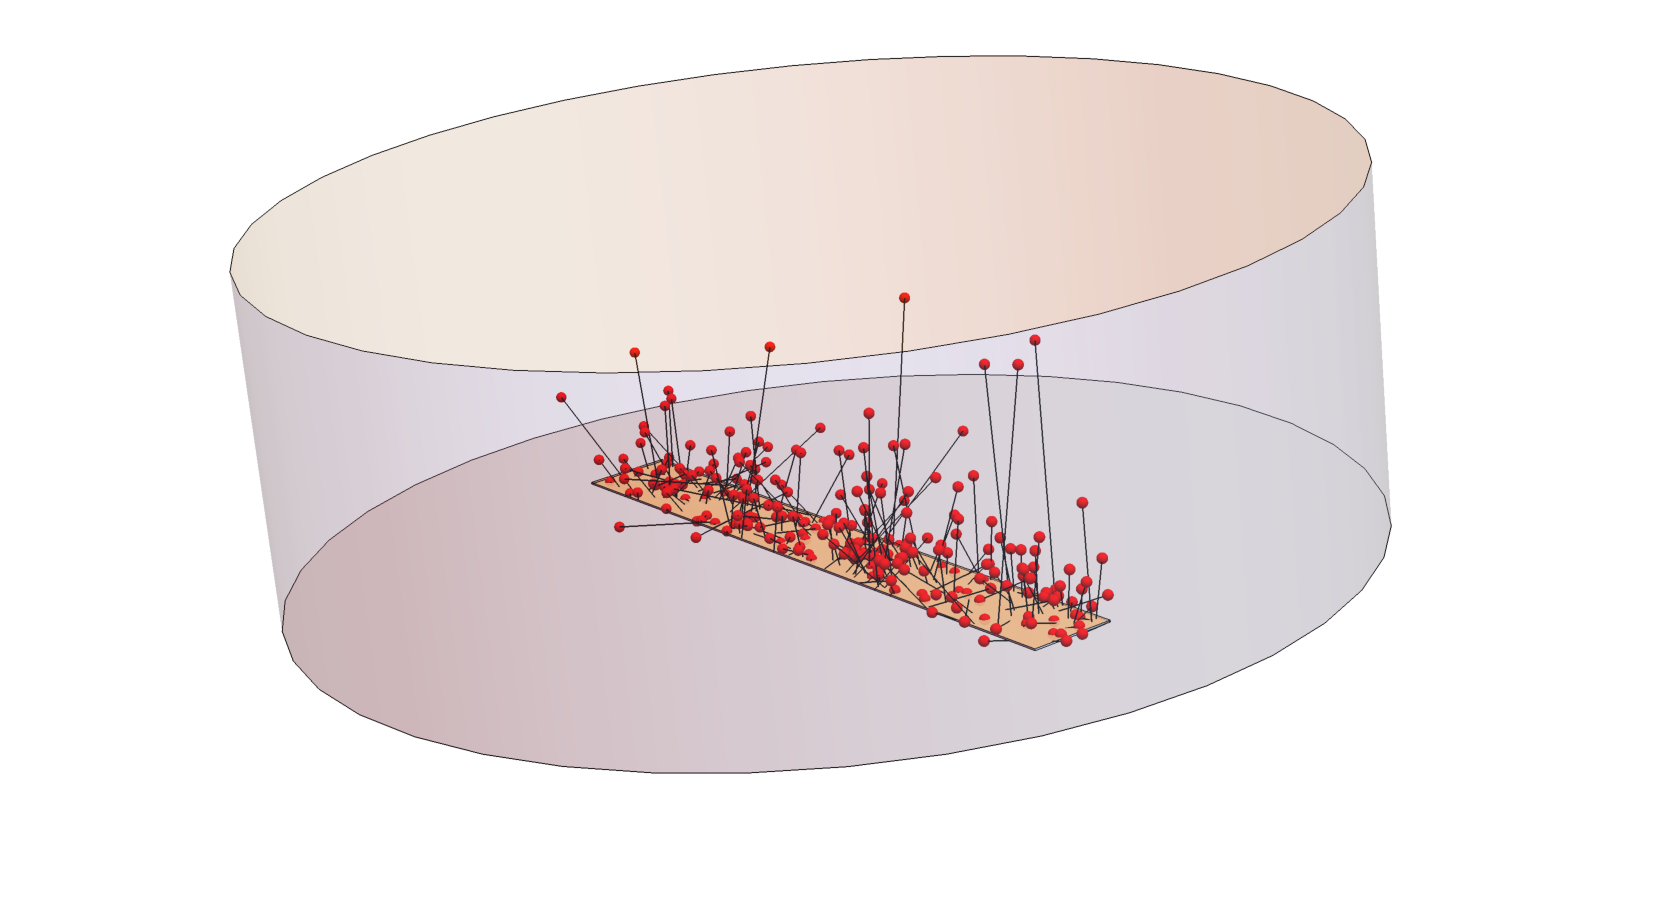
\includegraphics[width=1\linewidth]{Vis_500_1} \\ b)}
\end{minipage}
\caption{a) Точки рождения $\gamma$-квантов, b) <<Ёжик>>, $N = 500$}
\label{}
\end{figure}

\newpage
\begin{figure}[htbp]
  \centering
  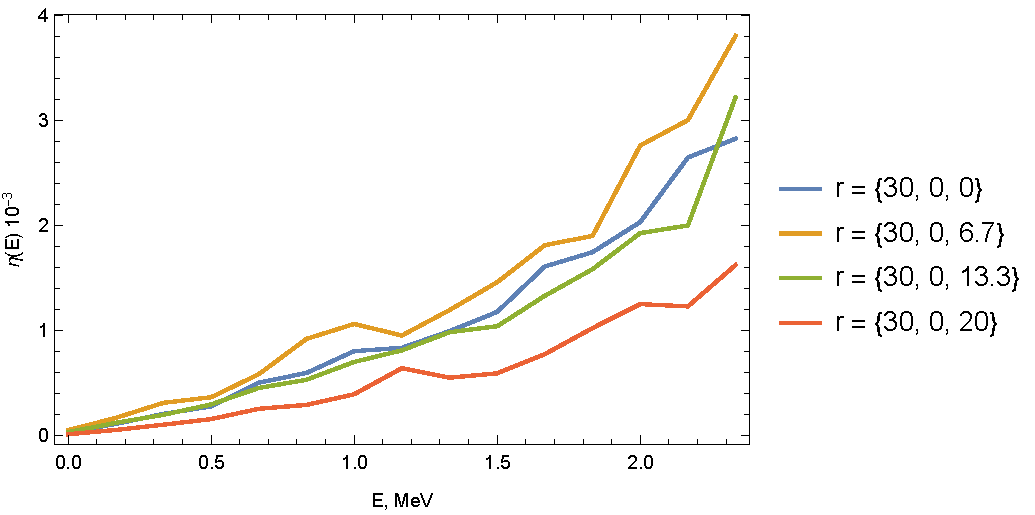
\includegraphics[width=0.95\linewidth]{10k_1}
  \caption{Распределения плотности потока рассеянных
квантов при детекторах, расположенных вдоль направляющей, $N = 10000$}\label{}
\end{figure}

\begin{figure}[htbp]
  \centering
  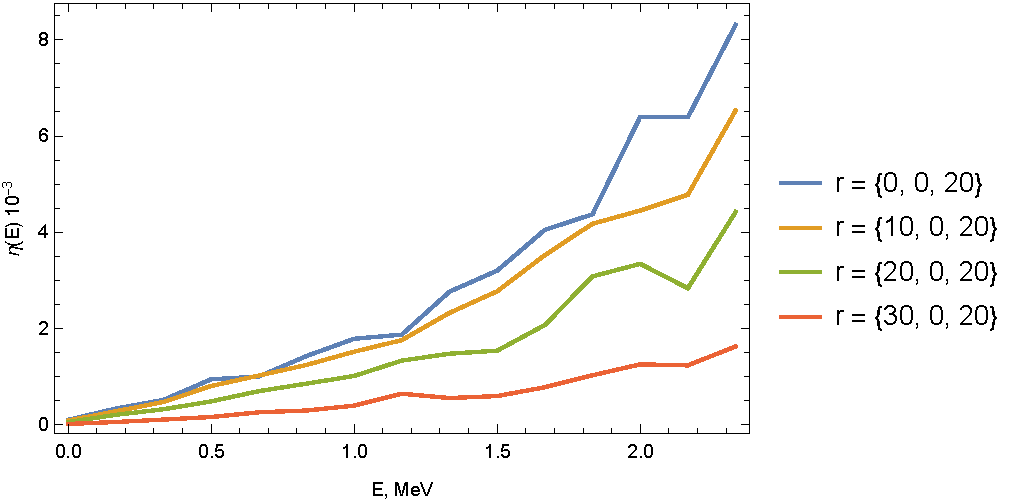
\includegraphics[width=0.95\linewidth]{10k_2}
  \caption{Распределения плотности потока рассеянных
квантов при детекторах, расположенных вдоль радиуса, параллельного стороне $a$ прямоугольника, $N = 10000$}\label{}
\end{figure}

\newpage
\begin{figure}[htbp]
  \centering
  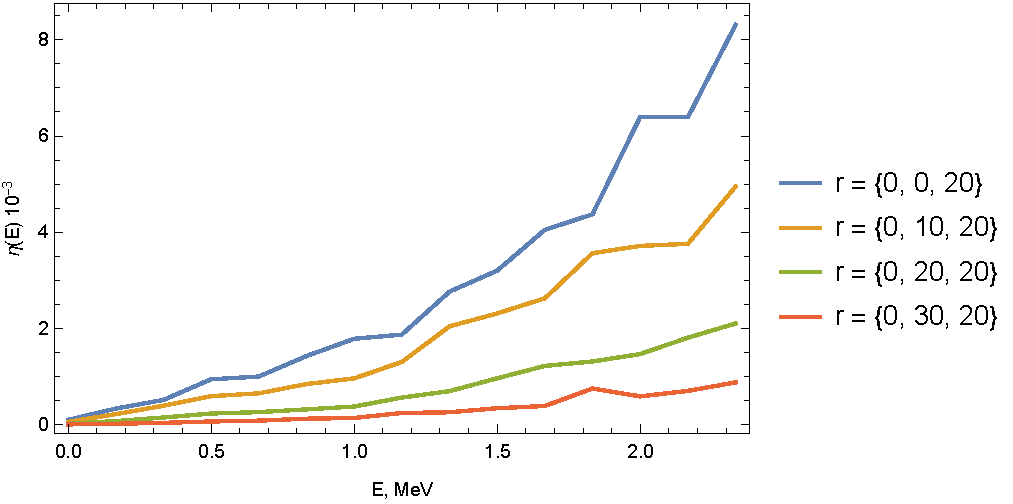
\includegraphics[width=0.95\linewidth]{10k_3}
  \caption{Распределения плотности потока рассеянных
квантов при детекторах, расположенных вдоль радиуса, параллельного стороне $b$ прямоугольника, $N = 10000$}\label{}
\end{figure}

\begin{figure}[htbp]
  \centering
  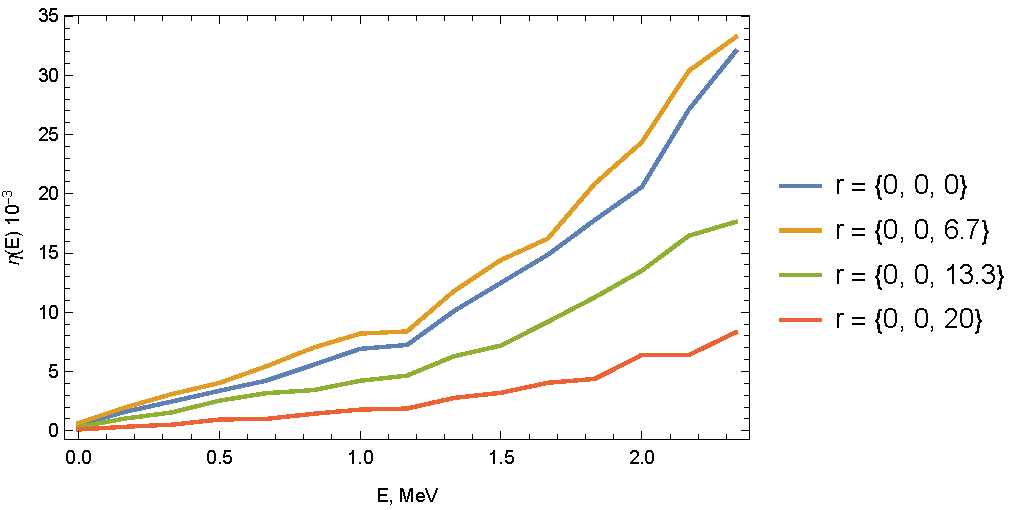
\includegraphics[width=0.95\linewidth]{10k_4}
  \caption{Распределения плотности потока рассеянных
квантов при детекторах, расположенных вдоль оси цилиндра, $N = 10000$}\label{}
\end{figure}

\newpage
\begin{figure}[htbp]
  \centering
  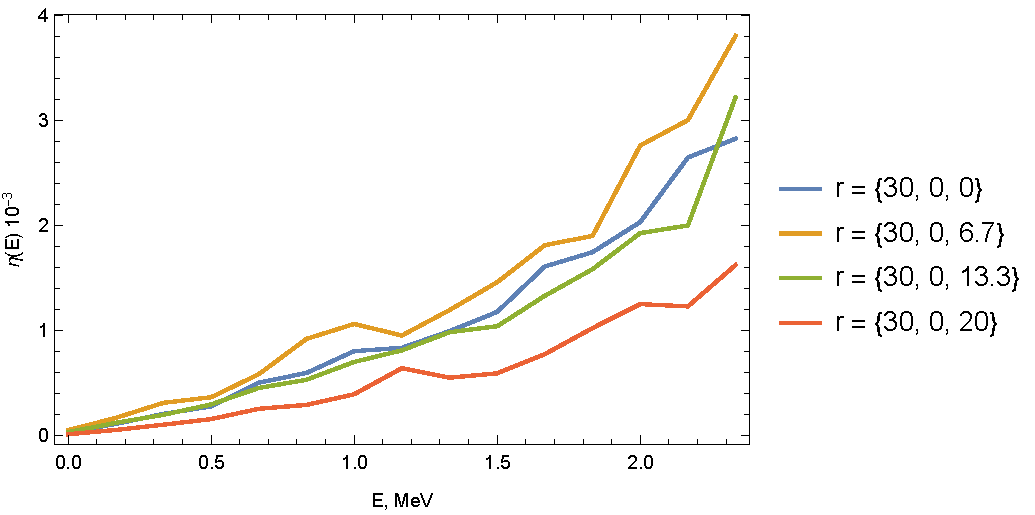
\includegraphics[width=0.95\linewidth]{50k_1}
  \caption{Распределения плотности потока рассеянных
квантов при детекторах, расположенных вдоль направляющей, $N = 50000$}\label{}
\end{figure}

\begin{figure}[htbp]
  \centering
  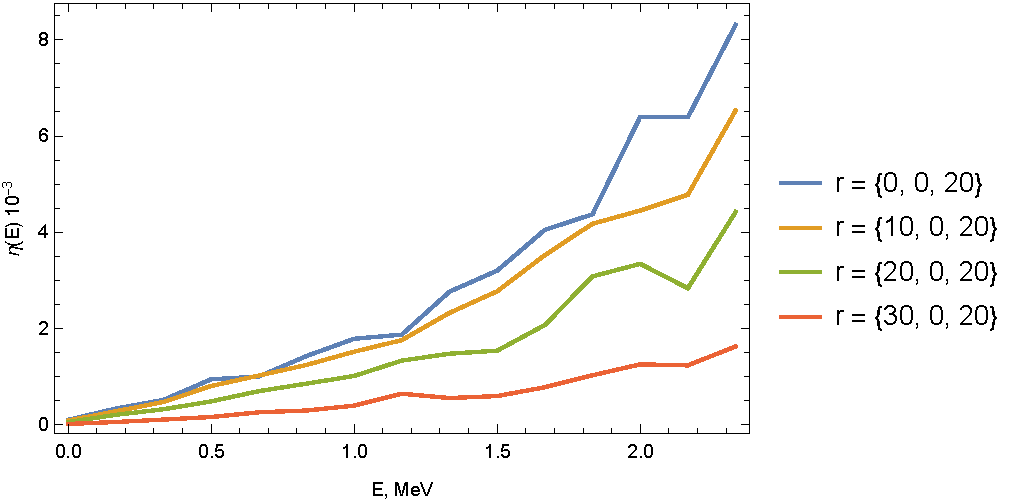
\includegraphics[width=0.95\linewidth]{50k_2}
  \caption{Распределения плотности потока рассеянных
квантов при детекторах, расположенных вдоль радиуса, параллельного стороне $a$ прямоугольника, $N = 50000$}\label{}
\end{figure}

\newpage
\begin{figure}[htbp]
  \centering
  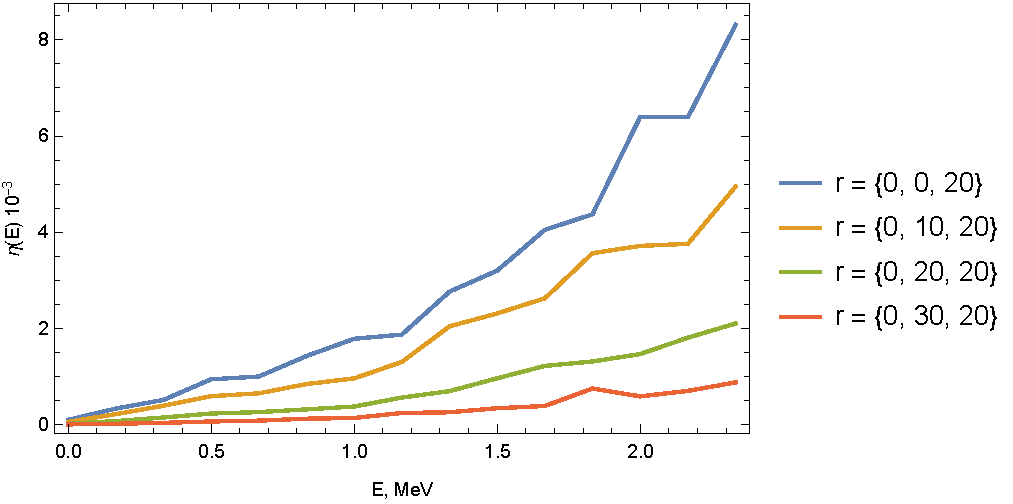
\includegraphics[width=0.95\linewidth]{50k_3}
  \caption{Распределения плотности потока рассеянных
квантов при детекторах, расположенных вдоль радиуса, параллельного стороне $b$ прямоугольника, $N = 50000$}\label{}
\end{figure}

\begin{figure}[htbp]
  \centering
  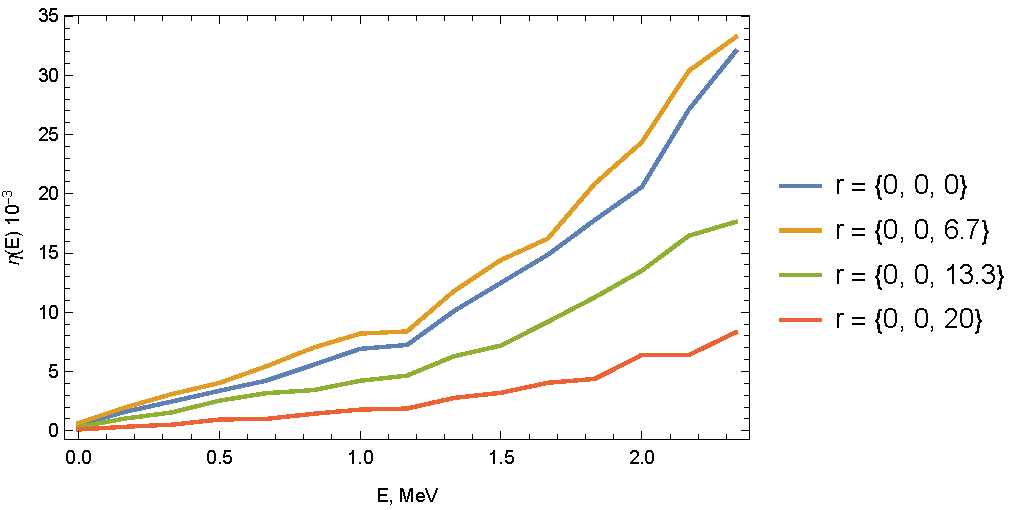
\includegraphics[width=0.95\linewidth]{50k_4}
  \caption{Распределения плотности потока рассеянных
квантов при детекторах, расположенных вдоль оси цилиндра, $N = 50000$}\label{}
\end{figure}

\newpage
\section{Вывод}
\noindent Методом Монте-Карло получены распределения плотности потоков рассеянных квантов при различных расположениях детекторов и различных количествах $\gamma$-квантов $N$. Наибольшая плотность потока наблюдается на детекторе с координатами $\left(0,0,\frac{20}{3}\right)$, наименьшая -- на детекторах, расположенных вблизи верхнего основания цилиндра.

\end{document} 